%% SECTION 8: EMPIRICAL VALIDATION
%% ============================================================
\section{Preliminary Learnability and Profile-Adherence Evidence}

\textbf{Claim scoped to this section: canonical data is learnable and can enforce target-profile adherence.} There is prior evidence that code model performance benefits heavily from data quality: Arctic-SnowCoder-1.3B used 555B tokens in staged data refinement and beat or matched models trained on much larger token budgets~\cite{arcticSnowCoder}. The phi-1 work showed that high-quality ``textbook'' data can produce remarkably capable small models~\cite{phi1}.

To test whether canonical-translated data produces healthy convergence, we ran a quantized low-rank adaptation (QLoRA) fine-tuning experiment on Qwen2.5-Coder-14B-Instruct~\cite{qlora,qwenCoder} using 64,088 canonically translated agentic coding trajectories (57,688 train, 6,400 validation). The dataset consists of verified multi-turn coding sessions where an agent reads a real GitHub issue, explores the codebase, applies a fix, and passes automated tests, then translates the trajectory through the canonical porting pipeline to align with the target limited-stack profile.

Training ran for 7,106 steps on a single NVIDIA RTX~3090 (24\,GB) over approximately three days. Key hyperparameters: LoRA rank $r{=}16$, $\alpha{=}32$, learning rate $2{\times}10^{-5}$ with constant-with-warmup schedule, effective batch size $1{\times}8$ gradient accumulation, maximum sequence length 2,048 tokens, 4-bit NF4 quantization with double quantization.

\begin{table}[t]
\caption{Pilot Configuration}
\label{tab:pilotconfig}
\centering
\footnotesize
\begin{tabularx}{\columnwidth}{p{0.34\columnwidth}X}
\toprule
Field & Value \\
\midrule
Base model & Qwen2.5-Coder-14B-Instruct \\
Adaptation & QLoRA, rank 16, alpha 32, 4-bit NF4, double quantization \\
Data & 64,088 translated trajectories; 57,688 train / 6,400 validation \\
Steps & 7,106 training steps; 711 validation evaluations \\
Sequence length & 2,048 tokens \\
Hardware & Single NVIDIA RTX 3090, 24\,GB \\
Forbidden marker metric & Average presence of off-profile markers such as Python \texttt{def}, Go \texttt{func}, and Java \texttt{public class} under target-profile service prompts \\
\bottomrule
\end{tabularx}
\end{table}

\begin{figure*}[t]
  \centering
  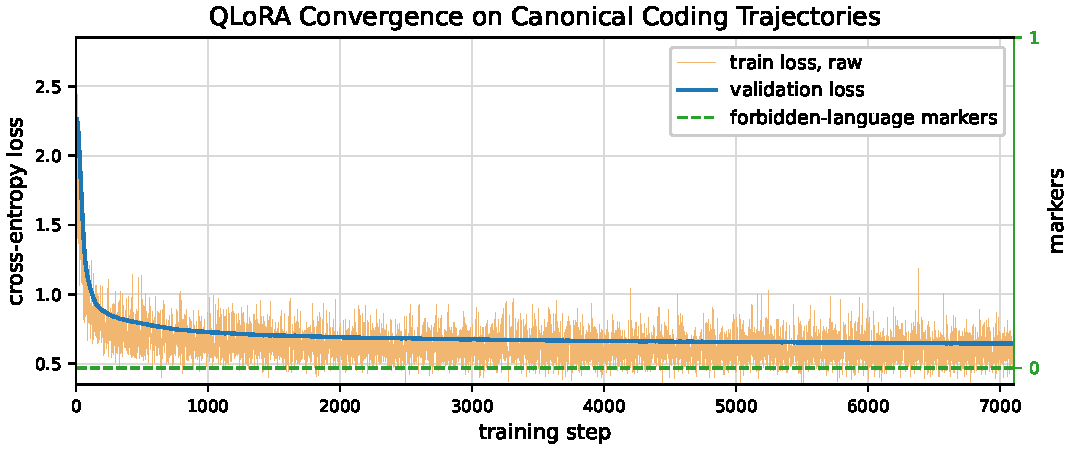
\includegraphics[width=\textwidth]{figures/convergence_plot.pdf}
  \caption{Raw training and validation loss convergence for QLoRA fine-tuning of Qwen2.5-Coder-14B on 64,088 canonically translated trajectories. The figure shows the real per-step training log after restart de-duplication: 7,106 training steps and 711 validation evaluations. Training loss starts at 2.707 and ends at a raw final value of 0.419. Validation loss drops from 2.261 at step 10 to 0.646 at step 7,106, with a minimum of 0.644 at step 6,780. Zero forbidden-language markers were recorded across all evaluation checkpoints. The vector figure is generated from raw per-step training logs and evaluation telemetry only.}
  \label{fig:convergence}
\end{figure*}

Figure~\ref{fig:convergence} shows the convergence curve generated from raw training telemetry. After restart de-duplication, the run contains 7,106 training steps and 711 validation evaluations. Raw training loss drops from 2.707 at step 1 to 0.419 at step 7,106. Validation loss drops from 2.261 at step 10 to 0.646 at step 7,106, closely tracking the raw training curve throughout. Two observations are significant:

\begin{enumerate}
\item \textbf{No visible train/validation divergence.} Raw training and validation losses fall together through the run, with validation ending at 0.646 after consuming 100\% of the training data. By contrast, raw open-source coding data typically requires aggressive deduplication: The Stack v2 reduced from 67.5\,TB to 32.1\,TB (52\% deduplication) and then to 2.4\,TB after quality filtering---a 96.4\% reduction.

\item \textbf{Zero forbidden-language violations.} Throughout training, evaluation checkpoints measured off-profile markers (Python \texttt{def}, Go \texttt{func}, Java \texttt{public class}, etc.) in model outputs prompted with target-profile service tasks. All 711 evaluation checkpoints recorded zero markers, indicating that canonical fine-tuning successfully steered the model toward the target profile.
\end{enumerate}

\begin{table}[t]
\caption{What the Pilot Proves and Does Not Prove}
\label{tab:pilotlimits}
\centering
\footnotesize
\begin{tabularx}{\columnwidth}{p{0.32\columnwidth}X}
\toprule
Status & Claim \\
\midrule
Shows & Canonical translated trajectories are learnable under this parameter-efficient adaptation setup. \\
Shows & The measured forbidden-language markers can be suppressed in the evaluation prompts. \\
Does not show & Behavior preservation, full stack correctness, held-out accepted-change success, or lower cost per verified change. \\
Does not show & Tokens-to-target reduction versus raw trajectories; that requires paired scaling curves from the same task lineage. \\
\bottomrule
\end{tabularx}
\end{table}

These results provide early evidence that canonical data is learnable under this parameter-efficient adaptation setup. They do not yet prove behavior preservation, cost-per-correct-change reduction, or 100B replacing 1T. Those require the full evaluation protocol described in Section~\ref{sec:eval}.

%% ============================================================
